\question[10] In the circuit shown in the figure, all of the wires are made of Nichrome, but one wire is very thin and the others are thick.

\begin{center}
	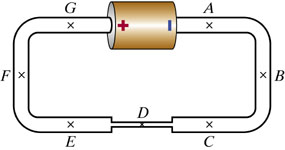
\includegraphics[width=.6\textwidth]{ch18q1.jpg}
\end{center}

Which of the following statements about this circuit are true? (Check all that apply)
\begin{todolist}
	\item The magnitude of the electric field at location G is smaller in this circuit than it would be if all the wires were thick.
	\item Fewer electrons per second pass location E than location C.
	\item The electron current in this circuit is less than the electron current would be if all the wires were thick.
	\item The electron current is the same at every location in this circuit.
	\item The magnitude of the electric field at location D is larger than the magnitude of the electric field at location G.
	\item The magnitude of the electric field is the same at every location in this circuit.
	\item The battery alone creates the electric field at every point in the circuit.
\end{todolist}